\documentclass[crop,tikz,10pt]{standalone}
\usepackage{tikz}
	\usetikzlibrary{shapes}
	\usetikzlibrary{automata}
	\usetikzlibrary{arrows}
	\usetikzlibrary{backgrounds}
	\usetikzlibrary{calc}
	\usetikzlibrary{positioning}
	\usetikzlibrary{patterns}
	\usetikzlibrary{decorations.pathmorphing}
	\usetikzlibrary{decorations.pathreplacing}

\usepackage[scaled]{helvet}
\renewcommand{\familydefault}{\sfdefault}

\usepackage{booktabs}
\usepackage{bm}
\usepackage{mhchem}
\usepackage{siunitx}
\usepackage{xcolor}
    \definecolor{TUMOrange}{RGB}{227, 114, 34}
    \definecolor{TUMBlueDark}{RGB}{0, 82, 147}

\input{../../../../resources/latex/_symbols.qmd}

\begin{document}

\newcommand{\n}[1]{\begin{tabular}{c}#1\end{tabular}}
\renewcommand{\vec}[1]{\boldsymbol{\mathbf{#1}}}

\pgfdeclarelayer{background}
\pgfdeclarelayer{foreground}

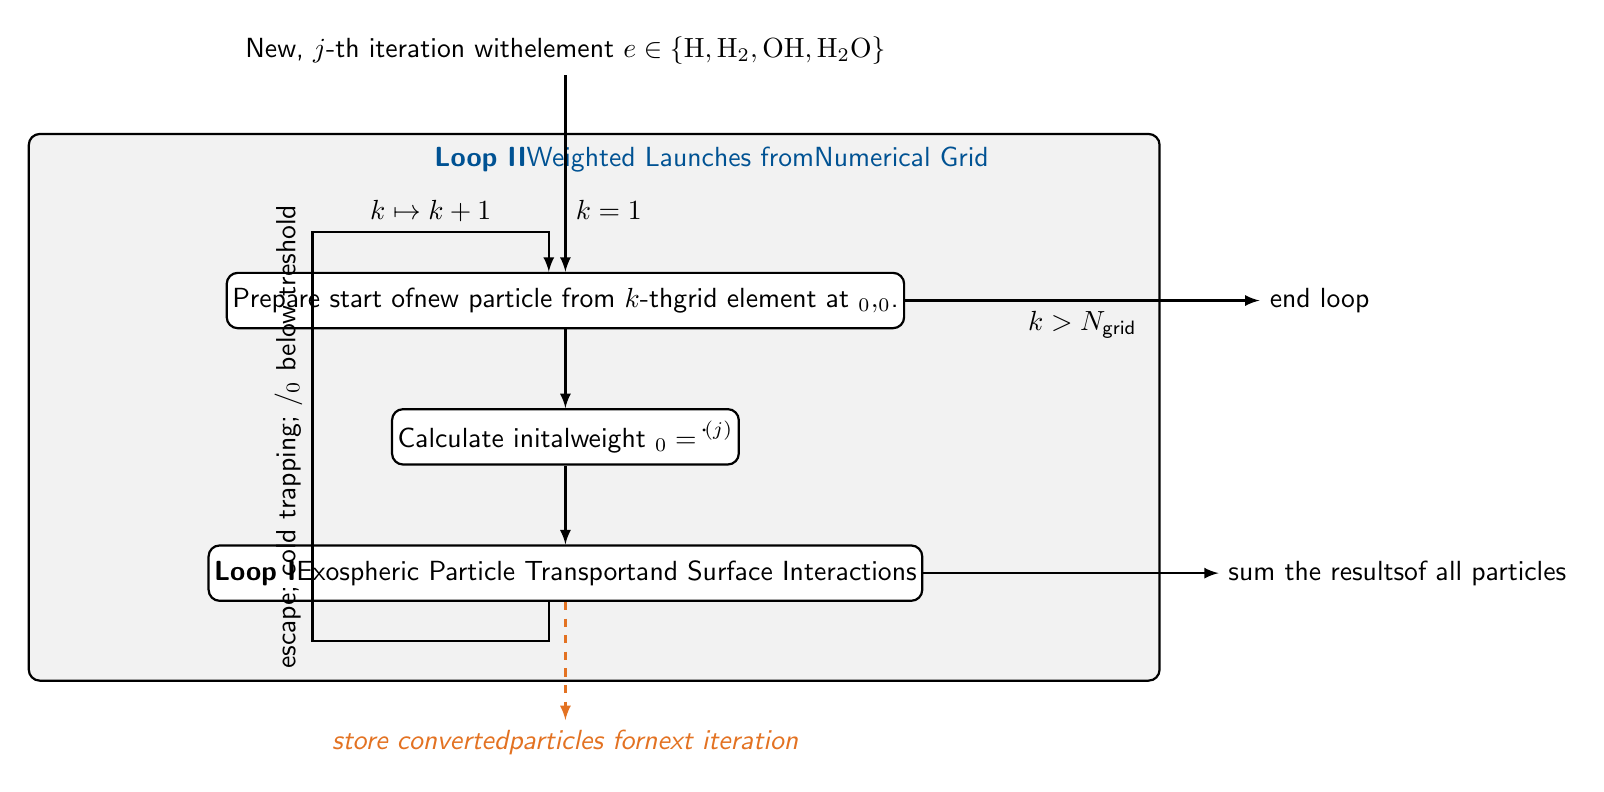
\begin{tikzpicture}[
    main/.style={draw, thick, rounded corners=4pt, inner sep=2pt, minimum size=20pt, minimum width=25pt, fill=white},
]

    %::. main nodes
    \node[main] (LOOPI) at (0,0) {\n{\textbf{Loop I} \\ Exospheric Particle Transport \\ and Surface Interactions}};
    \node[main, above = of LOOPI] (W0) {\n{Calculate inital \\ weight $\weight_0 = \dot{\source}^{(j)}$}};
    \node[main, above = of W0] (PREP) {\n{Prepare start of \\ new particle from $k$-th \\ grid element at $\sphericalCoordinateAzimuth_0, \sphericalCoordinateElevation_0$.}};
    \node[right = 3.75 of LOOPI] (SUM) {\n{sum the results \\ of all particles}};

    %::. main connections
    \draw[-latex, thick] (W0.270) -- (LOOPI.90);
    \draw[-latex, thick] (PREP.270) -- (W0.90);
    \draw[-latex, thick] (LOOPI.240) -- +(0,-0.5) -| ($(PREP.120) + (-3,0.5)$) node[near end, rotate=90, left, above] {escape; cold trapping; $\weight/\weight_0$ below treshold} -| (PREP.120) node[near start, above] {$k\mapsto k+1$};
    \draw[-latex, thick] (LOOPI.0) -- (SUM.180);

    \draw[-latex, thick] (PREP.0) -- +(4.5,0) node[midway, below]{$k > N_\text{grid}$} node[at end, right] {end loop};

    %::. conversion node from Loop I
    \node[below = 1.5 of LOOPI, text=TUMOrange] (STORE) {\textit{\n{store converted \\ particles for \\ next iteration}}};
    \draw[-latex, thick, dashed, TUMOrange] (LOOPI.270) -- (STORE.90);

    %::. input connection
    \draw[latex-, thick] (PREP.90) -- +(0,2.5) node[midway, right, yshift=-13px]{$k=1$} node[at end, above] {\n{New, $j$-th iteration with \\ element $e \in \left\{\ce{H}, \ce{H2}, \ce{OH}, \ce{H2O}\right\}$}};

    %::. background loop node
    \begin{pgfonlayer}{background}
        \draw[thick, fill=white!95!black, rounded corners=4pt] ($(PREP.north west) + (-2.5,1.75)$) rectangle ($(LOOPI.south east) + (3, -1)$);
        \node[anchor=north east, text=TUMBlueDark] at ($(PREP.90) + (5.5, 1.7)$) {\n{\textbf{Loop II} \\ Weighted Launches from \\ Numerical Grid}};
    \end{pgfonlayer}
\end{tikzpicture}

\end{document}